\section{39 - MAT - FA 2.5, AN 4.3, FA 1.5,  - Baumwachstum - Matura 2013/14 1. Nebentermin}

\begin{langesbeispiel} \item[0] %PUNKTE DES BEISPIELS
				Beim Wachstum von Bäumen wird die Zunahme der Höhe, des Durchmessers, der Grundfläche, des Volumens und der Baumkronenhöhe des Baumes beobachtet. 
				
				Die untenstehende Abbildung zeigt einen typischen Verlauf des Graphen einer Wachstumsgeschwindigkeitsfunktion von Bäumen. Die vier eingezeichneten Punkte markieren Wendepunkte des Graphen der Wachstumsgeschwindigkeitsfunktion $i$. 
				
				Beim Höhenwachstum des Baumes werden vier Phasen unterschieden. Auf die Jugendphase $J\,\,(0\leq t \leq t_1)$ folgt die Hauptphase $H\,\,(t_1\leq t\leq t_2)$, darauf folgt die Altersphase $A\,\,(t_2\leq t\leq t_3)$ und schließlich die Senilitätsphase $S$. $t$ ist das Lebensalter des Baumes in Jahren. $i(t)$ wird in Metern pro Jahr angegeben.

				\begin{center}\resizebox{0.8\linewidth}{!}{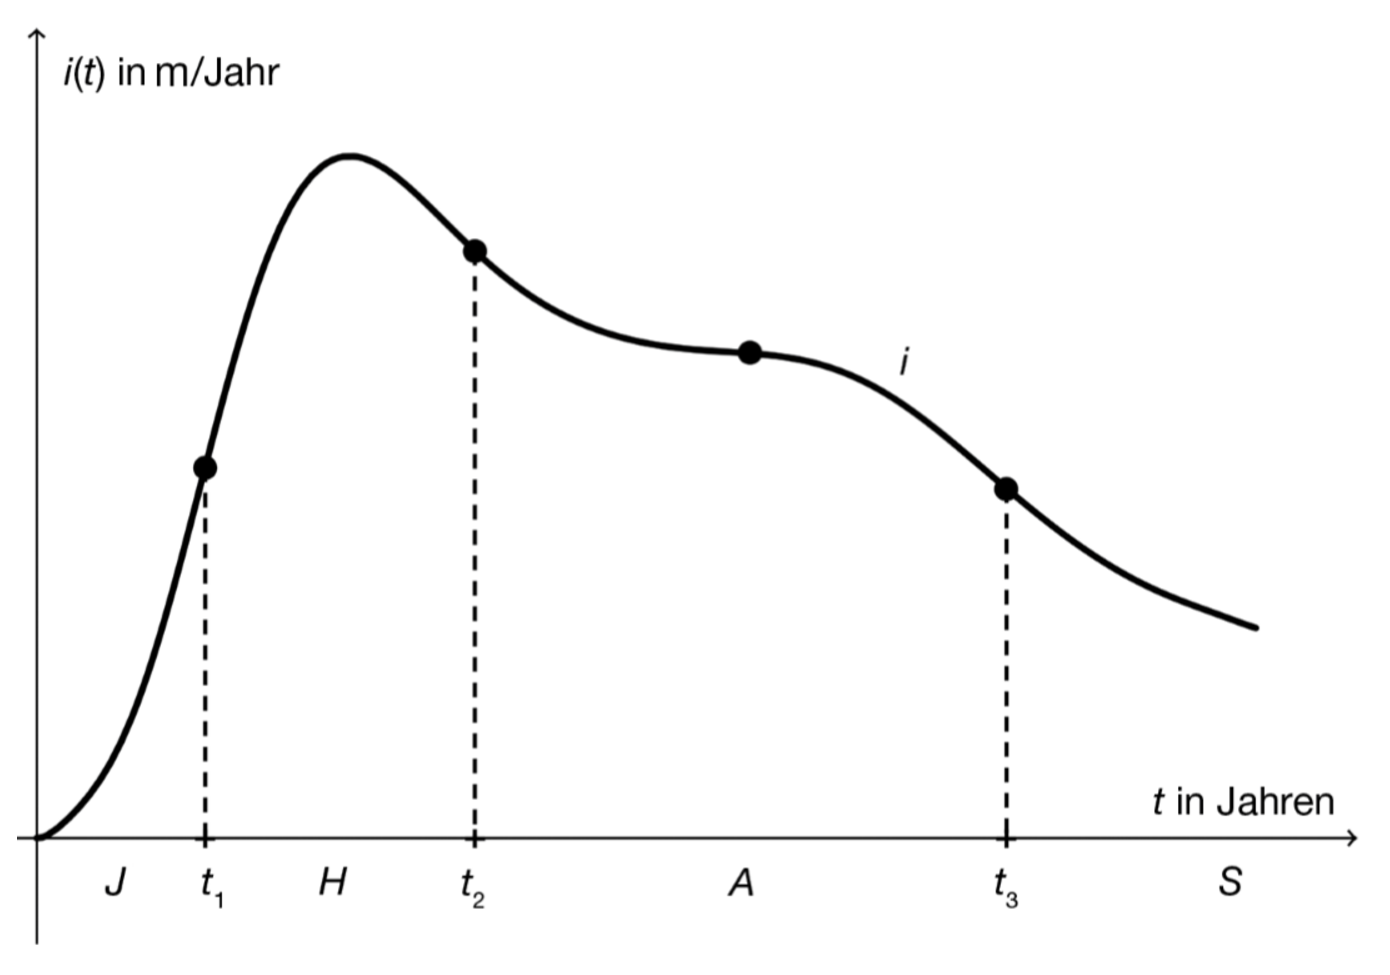
\includegraphics{../_database/Bilder/Bild39-1.eps}}\end{center}
				
				\begin{singlespace}
\begin{tiny}
(Quelle: http://www.wsl.ch/forest/waldman/vorlesung/ww\textunderscore tk32.ehtml $[21.05.2014]$ (adaptiert)) 
\end{tiny}
\end{singlespace}


\subsection{Aufgabenstellung:}
\begin{enumerate}
	\item Bestimme anhand der Abbildung, in welcher der vier Wachstumsphasen sich ein längerer Zeitraum befindet, in welchem die Höhe des Baumes annähernd linear zunimmt, und begründe deine Auswahl!
	
	Gib unter Verwendung der Wachstumsgeschwindigkeitsfunktion $i$ einen mathematischen Ausdruck an, der die Höhe des Baumes am Beginn der Senilitätsphase (also zum Zeitpunkt $t_3$) beschreibt!
					
\item Markiere in der nachstehenden Abbildung diejenige Stelle $t^*$ auf der $t$-Achse (in der Hauptphase $H$), für die $i'(t^*)=0$ gilt! Formuliere eine Aussage über das Höhenwachstum des Baumes an der Stelle $t^*$!

\begin{center}\resizebox{0.8\linewidth}{!}{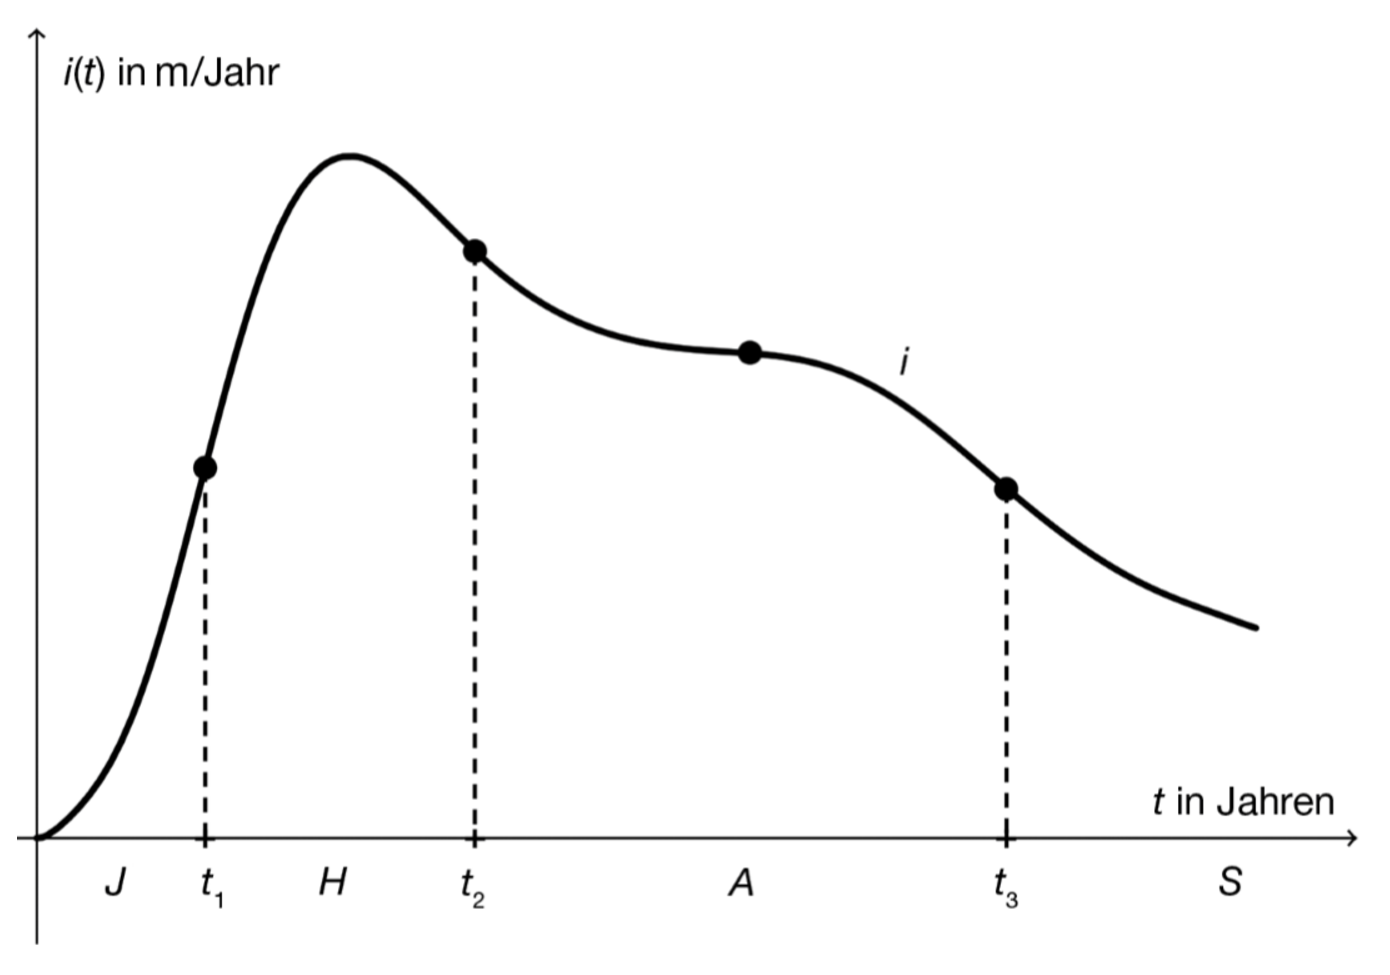
\includegraphics{../_database/Bilder/Bild39-1.eps}}\end{center}

Während der Jugendphase ist die Wachstumsgeschwindigkeitsfunktion $i$ monoton steigend, während der Altersphase ist $i$ monoton fallend. Interpretiere dieses Monotonieverhalten im Hinblick auf das Höhenwachstum des Baumes!
						\end{enumerate}\leer
				
\antwort{
\begin{enumerate}
	\item \subsection{Lösungserwartung:} 
	
	Im mittleren Bereich der Altersphase nimmt die Höhe des Baumes annähernd linear zu, weil der Höhenzuwachs pro Jahr annähernd konstant ist.
	
	Höhe des Baumes am Beginn der Senilitätsphase: $\int^{t_3}_0{i(t)}$d$t$
	 	
	\subsection{Lösungsschlüssel:}
	\begin{itemize}
		\item  Ein Punkt für die Nennung der Altersphase (bzw. die Markierung der betreffenden Stelle im Graphen) und die sinngemäß richtige Begründung, dass die Höhe des Baumes dann linear zunimmt, wenn $i$ waagrecht verläuft, d.h. der Höhenzuwachs konstant ist.
		\item Ein Punkt für das richtige Anschreiben des Integrals (inkl. Grenzen und Integrationsvariable).
	\end{itemize}
	
	\item \subsection{Lösungserwartung:}
			
		\begin{center}\resizebox{0.8\linewidth}{!}{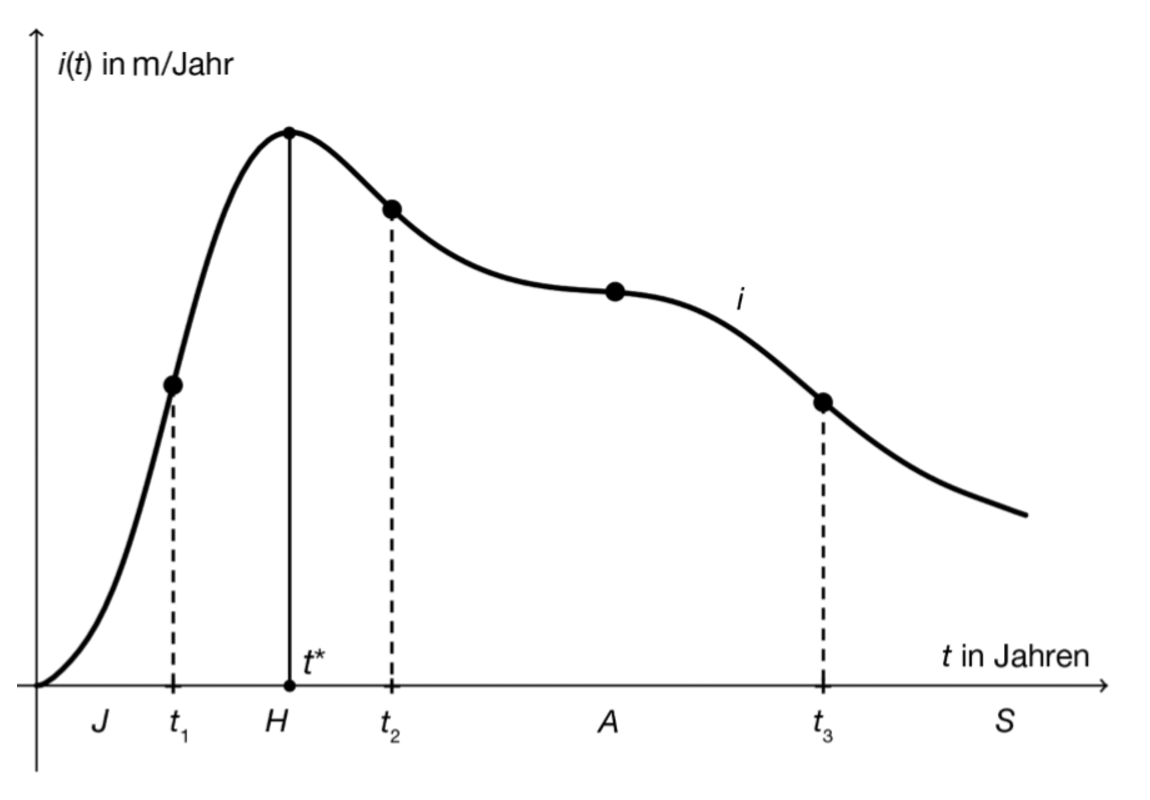
\includegraphics{../_database/Bilder/Bild39-2.eps}}\end{center}
		
		Zu diesem Zeitpunkt $(t^*)$ ist die Wachstumsgeschwindigkeit des Baumes größer als zu den Zeitpunkten davor und danach.
		
		Solange $i$ monoton steigt (Jugendphase), wächst der Baum immer schneller, d.h., die Höhenzunahme pro Jahr wird größer. Wenn $i$ monoton fällt (Altersphase), nimmt die Wachstumsgeschwindigkeit ab, d.h., der Baum wächst immer langsamer.
		
	\subsection{Lösungsschlüssel:}
	
\begin{itemize}
	\item Ein Punkt für die richtige Kennzeichnung der Maximumstelle und für eine sinngemäß richtige Interpretation dieses Zeitpunktes. Die Maximumstelle muss (auf der $t$-Achse!) erkennbar gekennzeichnet sein. Aus der formulierten Aussage muss klar hervorgehen, dass der Baum zu diesem Zeitpunkt am schnellsten wächst.
	\item Ein Punkt für eine (sinngemäß) korrekte Interpretation des Monotonieverhaltens von $i$ im Hinblick auf das Baumwachstum.
\end{itemize}
\end{enumerate}}
		\end{langesbeispiel}